\begin{frame}{Diagnóstico e Tratamento}
    \begin{block}{}
    A paciente foi submetida a uma laparotomia exploradora. 
    \end{block}
    \vspace{5mm} 
    Foi evidenciado 1.5 L de secreção mucopurulenta na cavidade abdominal.\vspace{5mm}
    E encontrando um divertículo de Meckel perfurado de aproximadamente 2-3 cm de comprimento, localizado a 70 cm da junção íleo-cecal, na borda antimesentérica.
\end{frame}

\begin{frame}{Diagnóstico e Tratamento}
    \begin{figure}
        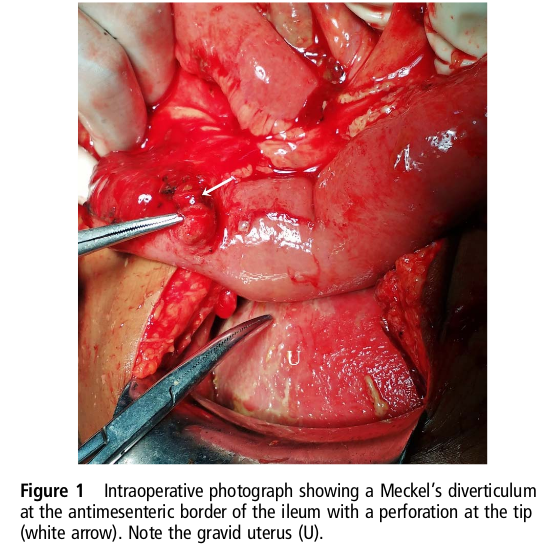
\includegraphics[width=220px]{img/foto.png}
    \end{figure}
\end{frame}


\begin{frame}{Diverticulo de Meckel}
    O divertículo de Meckel é a anomalia congênia do trato gastrointestial mais comum. Presente em 2 a 4\% da população.\vspace{5mm}
    
    As complicações mais comums são:
        \begin{itemize}
            \item Obstrução - 36,5\%
            \item Intussuscepção - 13,7\%
            \item Inflamação ou diverticulite - 12,7\%
            \item Hemorragia - 11,8\%
            \item Neoplasia - 3,2\%
            \item Fístula - 1,7\%
        \end{itemize}
\end{frame}

\begin{frame}{Diverticulo de Meckel}
    O tratamento do divertículo de Meckel em gestantes é o mesmo para pacientes não gestantes. \vspace{5mm}
    
    Consiste na cirurgia de diverticulotomia ou ressecção segmental seguida de anastomose.\vspace{5mm}
    
    Em casos de abdome séptico, a ileostomia é uma boa alternativa.
\end{frame}